\tikzset{every picture/.style={line width=0.75pt}} %set default line width to 0.75pt        

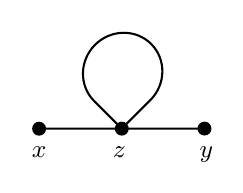
\begin{tikzpicture}[x=0.75pt,y=0.75pt,yscale=-1,xscale=1]
%uncomment if require: \path (0,300); %set diagram left start at 0, and has height of 300

%Shape: Tear Drop [id:dp9183665387422838] 
\draw   (233.52,74.66) .. controls (233.52,74.66) and (233.52,74.66) .. (233.52,74.66) .. controls (233.52,74.66) and (233.52,74.66) .. (233.52,74.66) .. controls (226.17,67.3) and (226.35,55.19) .. (233.94,47.6) .. controls (241.53,40.01) and (253.64,39.83) .. (260.99,47.18) .. controls (268.35,54.54) and (268.16,66.65) .. (260.58,74.24) .. controls (251.42,83.4) and (246.85,87.98) .. (246.84,87.97) .. controls (246.85,87.98) and (242.41,83.53) .. (233.52,74.66) -- cycle ;
%Shape: Circle [id:dp13521640125976497] 
\draw  [fill={rgb, 255:red, 0; green, 0; blue, 0 }  ,fill opacity=1 ] (244,87.97) .. controls (244,86.41) and (245.27,85.13) .. (246.84,85.13) .. controls (248.41,85.13) and (249.68,86.41) .. (249.68,87.97) .. controls (249.68,89.54) and (248.41,90.82) .. (246.84,90.82) .. controls (245.27,90.82) and (244,89.54) .. (244,87.97) -- cycle ;
%Straight Lines [id:da05158452588927387] 
\draw    (207,88) -- (286.68,87.95) ;
%Shape: Circle [id:dp5328590044568352] 
\draw  [fill={rgb, 255:red, 0; green, 0; blue, 0 }  ,fill opacity=1 ] (204.16,88) .. controls (204.16,86.43) and (205.43,85.16) .. (207,85.16) .. controls (208.57,85.16) and (209.84,86.43) .. (209.84,88) .. controls (209.84,89.57) and (208.57,90.84) .. (207,90.84) .. controls (205.43,90.84) and (204.16,89.57) .. (204.16,88) -- cycle ;
%Shape: Circle [id:dp11682351407883718] 
\draw  [fill={rgb, 255:red, 0; green, 0; blue, 0 }  ,fill opacity=1 ] (283.84,87.95) .. controls (283.84,86.38) and (285.11,85.11) .. (286.68,85.11) .. controls (288.25,85.11) and (289.53,86.38) .. (289.53,87.95) .. controls (289.53,89.52) and (288.25,90.79) .. (286.68,90.79) .. controls (285.11,90.79) and (283.84,89.52) .. (283.84,87.95) -- cycle ;

% Text Node
\draw (241,95.40) node [anchor=north west][inner sep=0.75pt]  [font=\small]  {$z$};
% Text Node
\draw (202,95.40) node [anchor=north west][inner sep=0.75pt]  [font=\small]  {$x$};
% Text Node
\draw (282.84,95.40) node [anchor=north west][inner sep=0.75pt]  [font=\small]  {$y$};


\end{tikzpicture}